\belowdisplayskip=12pt plus 3pt minus 9pt
\belowdisplayshortskip=7pt plus 3pt minus 4pt

\chapter{Background Research}
This chapter details the background research we have done in order to understand the Hopfield Neural Networks, realise their importance in various applications and to investigate the feasibility of our project.

\section{Attachment Theory}

One of the most interesting applications of the Hopfield Networks and Boltzmann Machines is related to modelling the Attachment Theory. This is a psychological study that describes the dynamics of long-term relationships between humans\cite{website:attachment_theory_wiki}. It focuses primarily on the type of attachment that an infant develops with the primary caregiver. There exist 2 main types of attachment: secure and insecure. Insecure patterns are further divided into insecure-avoidant, insecure-disorganised and insecure-resistant. The type of attachment developed by infants depends on the quality of care they have received\cite{website:attachment_theory_wiki}.

\subsection{Strange Situation Procedure}

%Just meantioned about it, since Abbas said we shouldn't go into detail here.
The classification of infants into the corresponding attachment type is formulated in the Strange Situation Procedure. The child is observed playing for 20 minutes while caregivers and strangers enter and leave the room, recreating the environment of the familiar and unfamiliar presence in most of the children's lives.\cite{website:attachment_patterns_wiki}

\section{Practical applications of Attractor Neural Networks}

%This should be expanded. Not sure what Abbas has in mind, but I believe our main motivation is not to model Attachment Theory.
Neural Networks have been successfully used in medical computing, in order to diagnose Parkinson's disease\cite{nets_parkinsons}. Other applications include facial recognition, which we have implemented for the purpose of this project, combinatorial problems such as the Travelling Salesman\cite{hopfield_laferriere}.
One practical application of the attractor neural networks, such as the Boltzmann machine, is the performance improvement of speech recognition software\cite{speech_nets}.


\section{Hopfield Networks}

%This section with Hopfield Networks has loads of sub-sections. We should consider adding some hierarchy.
The Hopfield Networks are a form of recurrent artificial neural networks invented by John Hopfield in 1982 \cite{hopfield_wiki}. It aims to store and retrieve information like the human brain. It basically consists of a complete graph of N neurons, each having a value of +1 or -1 associated to it. Since the graph is complete, each pair of neurons (i,j) is connected by an edge, having an associated weight \( w_{ij}\).

\subsection{Updating the Hopfield Network}

The network is able to update the values associated to neurons by adhering to certain simple rules. Updating can be performed in two different manners:
\begin{itemize}
 \item Synchronous: All nodes are updated at a time. This requires a central clock to the system in order to maintain synchronisation. This method is less realistic, since biological or physical systems lack a global clock that keeps track of time.
 \item Asynchronous: Only one node is updated at a time. A random node can be chosen as the next one to get updated, or otherwise a sequence of nodes can be imposed a-priori.
\end{itemize}

Assume N neurons = 1.. N, with values \(x_{i} = \pm1\). The updating of an individual node i is performed by first calculating a weighted sum of the neighbouring nodes, and then applying the sign function:

 \[x_{i} = sgn(\sum_{j=1}^{N}w_{ij}x_{j} + b_{i})\]

where \( b_{i} \) is a bias that we will consider to be equal to 0 for the purpose of this project.

Suppose the weight \( w_{ij}\) between neurons i and j is positive. Then, if the value of \( x_{j} \) is positive, then the term \( w_{ij}x_{j} \) will also be positive, and will drag the linear sum value to a positive value. This would mean that the neuron \( x_{i} \) would also be dragged towards a positive value. 

If updating is repeatedly performed, the network would eventually may converge to an attractor pattern under asynchronous updating, or it might sometimes cycle under synchronous updating. 

\subsection{Training using the Hebbian Rule}

The Hebbian theory has been introduced by Donald Hebb in 1949, in order to explain "associative learning", in which simultaneous activation of neuron cells leads to pronounced increases in synaptic strength between those cells \cite{hebb_wiki}. It is often summarised as "Neurons that fire together, wire together".

For the Hopfield Networks, this is implemented in the following manner, when learning p patterns:

\[ w_{ij}=\frac{1}{N}\sum_{\mu=1}^{p}\epsilon_{i}^\mu \epsilon_{j}^\mu \]

For pattern \(\mu\), if the bits corresponding to neurons i and j are equal, then the product  \( \epsilon_{i}^\mu \epsilon_{j}^\mu \) will be positive. This would, in turn, have a positive effect on the weight \(w_{ij} \) and the values of i and j will tend to become equal. The opposite happens if the bits corresponding to neurons i and j are different.

\subsection{Spurious Patterns}

Patterns that the network uses for training, called retrieval states, become attractors of the system. Repeated updates would eventually lead to convergence to one of the retrieval states. However, sometimes the network will converge to spurious patterns, that are different from the training patterns. 

A a linear combination of an odd number of stored patterns, in this case 3 patterns, would give us a spurious state:

\[ \epsilon_{i}^{mix} = \pm sgn(\pm \epsilon_{i}^{\mu_{1}} 
			         \pm \epsilon_{i}^{\mu_{2}}
			         \pm \epsilon_{i}^{\mu_{3}}) \]

However, we shall later on see that the probability of the network converging to these states is small, because of the tiny basin size. Furthermore, the Boltzmann Machine has the capacity of getting out of these spurious states, because of the probabilistic updating of the nodes.

\subsection{Energy Landscape}

One of Hopfield's most important contributions was to associate a Lyapunov, or energy function to the neural network. This is calculated as:

\[ E = -\frac{1}{2} \sum_{i,j=1}^{N}w_{ij}x_{i}x_{j} \]

The function decreases as the system gets updated until it reaches a local minimum, corresponding to an attractor.

% Inportenergy Landscape drawing from Lukasz
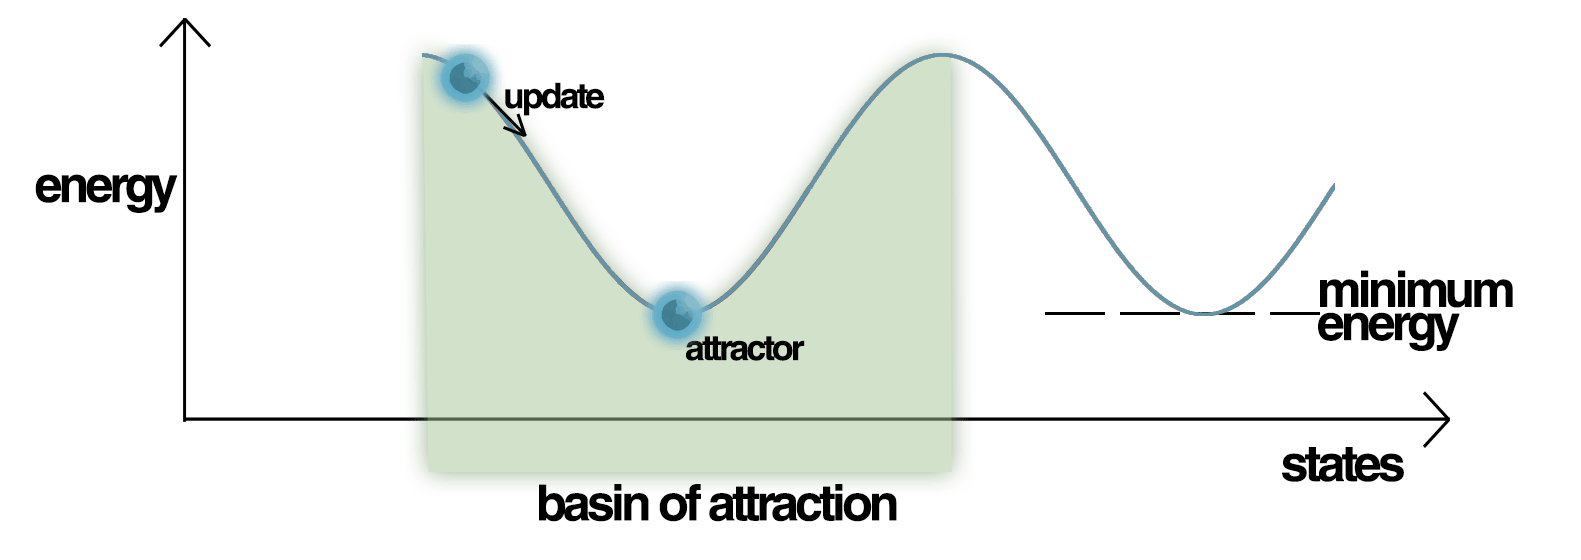
\includegraphics[scale=0.25]{energy_landscape.png}

\subsection{Stability and Capacity}

Concepts of stability and capacity are important in the analysis of Hopfield Networks. A neuron unit \( \epsilon_{i}^{\mu}\) is said to be stable if the update rule will not change its state. The mathematical condition for this is:

 \[x_{i} = sgn(\sum_{j=1}^{N}w_{ij}x_{j}) \]

Since we are using the Hebbian Rule, we can replace \(w_{ij}\) with
\(\sum_{\nu}\epsilon_{i}^{\nu}\epsilon_{j}^{\nu}\), resulting in:

\[ h_{i}^{\mu} = \frac{1}{N}\sum_{j} \sum_{\nu} \epsilon_{i}^{\nu}
						 \epsilon_{j}^{\nu}
						 \epsilon_{j}^{\mu}\]
 
 We will now isolate the contribution of neuron i, in order to get:
 
\[ h_{i}^{\mu} = \epsilon_{i}^{\nu} + \frac{1}{N}\sum_{j} \sum_{\nu\neq\mu} 			 					 \epsilon_{i}^{\nu}
						 \epsilon_{j}^{\nu}
						 \epsilon_{j}^{\mu}\]
 
 Now, the input for node i is made of two components: the first component depends on the node i itself, while the second component, called the \textbf{crosstalk term}, is directly dependent upon the neighbours of the node. 
 
 If we multiply the crosstalk term by \(-\epsilon_{i}^{\nu}\),  we get a quantity that will help us study the capacity:
 
 \[ C_{i}^{\nu}= -\epsilon_{i}^{\nu} \frac{1}{N}\sum_{j} \sum_{\nu\neq\mu} 			 			\epsilon_{i}^{\nu}
		       		 \epsilon_{j}^{\nu}
				 \epsilon_{j}^{\mu}\]
 
 If \( C_{i}^{\nu} \) is negative, then the cross-talk term has the same sign as unit i, and thus this value will not change \cite{lectureslides}. However, if \( C_{i}^{\nu} \) is positive and greater than 1, then \( \epsilon_{i}^{\nu}\) will change, so node i will become unstable. We will estimate the probability of \( C_{i}^{\nu} > 1 \)
 
 \textbf{UNFINISHED}
 
\subsection{Training using the Pseudo-Inverse Rule}

The pseudo-inverse rule makes use of the inverse of a matrix in order to perform the learning process. In contrast to the Hebbian Learning, it offers a higher capacity and performs better with correlated, linearly independent patterns. The weight matrix is computed as:

\[ w_{ij} = \frac{1}{N} \sum_{\mu\nu}\epsilon_{i}^\mu Q^{-1} \epsilon_{j}^\mu \]

In this case, Q is the overlap matrix:
\(  Q_{\mu\nu} = \frac{1}{N}\sum_{i}\epsilon_{i}^\mu \epsilon_{i}^\nu \)

%Locality and Incrementality
%I thought it would be best to be inserted here, since the reader has just been introduced to the second training rule, and can easily compare and reason out why these properties are useful
Now that we have introduced a second learning rule, it is worth mentioning a few desirable properties that neural network learning rules should aim to have. In Artificial Neural Networks, learning rules can be:
\begin{itemize}
 \item Local: each weight is updated using information available to neurons on either side of the connection.
 \item Incremental: new patterns can be learned without using information from the older patterns. When a new pattern is used for training, the new values for the weights only depend on the old values and on the bits of the pattern.
\end{itemize}

These properties are desirable, since learning becomes more biologically plausible. For example, since our brain is always learning new concepts, we can reason that learning is incremental. A learning system that would not be incremental would generally be trained only once, with a huge batch of training data.

It is important to mention that Hebbian Learning is both local and incremental, whereas the Pseudo-inverse learning rule is neither local nor incremental, since it depends upon the computation of an inverse matrix that contains information about all the patterns together.

\subsection{Training using the Storkey Rule}

The weight matrix of an attractor neural network is said to follow the Storkey learning rule if it obeys:

\[ w_{ij}^{\nu-1} = w_{ij}^{\nu-1}+
		    +\frac{1}{n}\epsilon_{i}^{\nu} \epsilon_{j}^{\nu} 
		    -\frac{1}{n}\epsilon_{i}^{\nu} h_{ji}^{\nu}
		    -\frac{1}{n}h_{ij}^{\nu} \epsilon_{i}^{\nu}
		    \]

where \( h_{ji}^{\nu} = \sum_{k=1,k\neq,j}^{n} w_{ik}^{\mu-1}\epsilon_{k}^{\mu} \) is a form of \emph{local field} \cite{storkey1997increasing} at neuron i.\\ 
		    
This rule is local, since the synapses take into account only neurons at their sides. This rule is slightly more powerful than the generalised Hebb rule, since it makes use of more information. Because of the action field, each neuron uses information from all the neighbours. As Storkey has showed in 1997, the capacity of the network trained with this rule is greater than compared to Hebbian rule \cite{storkey1997increasing}.


\subsection{Basins of Attraction}
%I think we should move the measurements for the basins of attraction in here.
A basin of attraction for a particular attractor a is defined as the set of all states that will eventually converge to a, under repeated update. Here, we are particularly interested in finding a way to measure the size of such a basin of attraction. A large basin size would provide stability for the attractor, since the states in the neighbourhood would converge to it. A small basin size for an attractor would mean that the network might never recall the pattern corresponding to that attractor.

